\documentclass{scrartcl}
\usepackage{tikz}
\usepackage{tcolorbox}
\usepackage{amsmath,amssymb}
\usepackage[top=2cm, bottom=2cm, left=2.5cm, right=2.5cm]{geometry}

\newcommand{\var}[1]{\text{\emph{#1}}}

\newcommand{\synencodingof}[1]{S\left(#1\right)} % Syntax encoding!
\newcommand{\stringof}[1]{\textit{"#1"}}

\newcommand{\rdf}{\mathrm{RDF}}
\newcommand{\mathrdftype}{\mathrm{rdf}\mathrm{type}}
\newcommand{\rdftype}{$\mathrm{rdf}:\mathrm{type}$}

\newcommand{\zerotuple}[1]{0_{#1}}
\newcommand{\onetuple}[1]{1_{#1}}

\newcommand{\truesymbol}{\mathrm{True}}
\newcommand{\falsesymbol}{\mathrm{False}}
\newcommand{\truthset}{\{\falsesymbol,\truesymbol\}}
\newcommand{\truthstate}{z}
\newcommand{\truthstateof}[1]{\truthstate_{#1}}
\newcommand{\ozset}{\{0,1\}}
\newcommand{\ozbasisset}{\{\fbasisat{\catvariable},\tbasisat{\catvariable}\}}

\newcommand{\setwithout}[2]{#1\backslash#2}
\newcommand{\setexcept}[1]{\backslash#1}
\newcommand{\whileSymbol}{$\mathrm{while}$}

\newcommand{\modspace}{\,\,\,\mathrm{mod}\,\,}

\newcommand{\uniquantwrtof}[2]{\forall{#1}:{#2}}
\newcommand{\existquantwrtof}[2]{\exists{#1}:{#2}}
\newcommand{\imppremhead}[2]{\left(#1\right)\Rightarrow\left(#2\right)}

\newenvironment{centeredscript}% Use for tnreason script language, lstlistings for python code!
{\begin{center}
     \begin{algorithmic}
         \hspace{1cm}}
{\end{algorithmic}\end{center}}

\newcommand{\inlinecode}[1]{\lstinline[language=Python]|#1|}

\newcommand{\algdefsymbol}{\leftarrow}
\newcommand{\proofrightsymbol}{"$\Rightarrow$"}
\newcommand{\proofleftsymbol}{"$\Leftarrow$"}
\newcommand{\defcols}{\,:\,} % in definitions of functions
\newcommand{\wcols}{\,:\,} % in definitions of sets
\newcommand{\ncond}{,\,} %next cond
\newcommand{\defspace}{\quad,\quad}
\newcommand{\andspace}{\quad\text{and}\quad}
\newcommand{\ifspace}{\text{if}\quad}
\newcommand{\elsetext}{\text{else}}
\newcommand{\stspace}{\quad \text{subject to} \quad}

\newcommand{\iosepline}{\vspace{0.5em} \hrule \vspace{0.5em}}

\newcommand{\distassymbol}{\sim}
\newcommand{\probtagtypeinst}[2]{\mathrm{P}^{#1}_{#2}}

\newcommand{\mprojectionsymbol}{\mathrm{M}}
\newcommand{\iprojectionsymbol}{\mathrm{I}}
\newcommand{\gainsymbol}{\mathrm{gain}}
\newcommand{\gradientsymbol}{\mathrm{grad}}
\newcommand{\greedysymbol}{\mathrm{greedy}}
\newcommand{\hubosymbol}{\mathrm{HUBO}}
\newcommand{\maximizationsymbol}{\mathrm{max}}

% Entropies
\newcommand{\entropysymbol}{\mathbb{H}}
\newcommand{\sentropyof}[1]{\entropysymbol\left[#1\right]}
\newcommand{\sentropyofwrt}[2]{\entropysymbol_{#2}\left[#1\right]}
\newcommand{\centropyof}[2]{\entropysymbol\left[#1,#2\right]}
\newcommand{\centropyofwrt}[3]{\entropysymbol_{#3}\left[#1,#2\right]}
\newcommand{\kldivsymbol}{\mathrm{D}_{\mathrm{KL}}}
\newcommand{\kldivof}[2]{\kldivsymbol\left[ #1 || #2 \right]}
\newcommand{\mutinfof}[2]{I\left(#1;#2\right)}
\newcommand{\condmutinfof}[3]{\mutinfof{#1}{#2|#3}}
\newcommand{\subspacedimof}[1]{\mathrm{dim}(#1)}

\newcommand{\subsphere}{\mathbb{S}}
\newcommand{\rr}{\mathbb{R}}
\newcommand{\nn}{\mathbb{N}}

\newcommand{\closureof}[1]{\overline{#1}}
\newcommand{\interiorof}[1]{{#1}^{\circ}}
\newcommand{\sbinteriorof}[1]{{\left(#1\right)}^{\circ}}

\newcommand{\difofwrt}[2]{\frac{\partial #1}{\partial #2}}
\newcommand{\difwrt}[1]{\difofwrt{}{#1}}
\newcommand{\gradwrt}[1]{\nabla_{#1}}
\newcommand{\gradwrtat}[2]{\nabla_{#1}|_{#2}}

\newcommand{\cardof}[1]{\left|#1\right|}
\newcommand{\absof}[1]{\left|#1\right|}

\newcommand{\imageof}[1]{\mathrm{im}\left(#1\right)}

\newcommand{\convhullof}[1]{\mathrm{conv}\left(#1\right)}
\newcommand{\cubeof}[1]{[0,1]^{#1}}
\newcommand{\dimof}[1]{\mathrm{dim}\left(#1\right)}
\newcommand{\spanof}[1]{\mathrm{span}\left(#1\right)}
\newcommand{\subspaceof}[1]{V^{#1}}

\newcommand{\argmin}{\mathrm{argmin}}
\newcommand{\argmax}{\mathrm{argmax}}

% Help functions
\newcommand{\chainingfunction}{h}
\newcommand{\chainingfunctionof}[1]{\chainingfunction\left(#1\right)}

\newcommand{\greaterthanfunction}[1]{\ones_{>#1}}
\newcommand{\greaterthanfunctionof}[2]{\greaterthanfunction{#1}\left(#2\right)}
\newcommand{\existquanttrafo}{\greaterthanfunction{0}}
\newcommand{\universalquanttrafo}{\greaterthanfunction{\inddim-1}}

\newcommand{\greaterzerofunction}{\greaterthanfunction{0}}
\newcommand{\greaterzeroof}[1]{\greaterzerofunction\left(#1\right)}
\newcommand{\equalzeroof}[1]{\ones_{\{0\}}\left(#1\right)}
\newcommand{\equaloneof}[1]{\ones_{\{0\}}\left(#1\right)}

\newcommand{\nonzerofunction}{\ones_{\neq0}}
\newcommand{\nonzeroof}[1]{\nonzerofunction\left(#1\right)}
\newcommand{\nonzerocirc}{\nonzerofunction\circ}

\newcommand{\valof}[1]{\mathrm{val}\left(#1\right)}

% Probability distributions
\newcommand{\expof}[1]{\mathrm{exp}\left[#1\right]}
\newcommand{\probtensor}{\mathbb{P}}
\newcommand{\probtensorof}[1]{\probtensor^{#1}}
\newcommand{\probtensorofat}[2]{\probtensor^{#1}\left[#2\right]}
\newcommand{\secprobtensor}{\tilde{\mathbb{P}}}
\newcommand{\secprobat}[1]{\secprobtensor[#1]}
\newcommand{\secprobwith}{\secprobat{\shortcatvariables}}

\newcommand{\probfamilyofat}[3]{\probofat{#1}{#2|#3}}
\newcommand{\membervariable}{Z}
\newcommand{\memberindex}{z}
\newcommand{\indexedmembervariable}{\membervariable=\memberindex}
\newcommand{\probfamilywith}{\probfamilyof{}{\shortcatvariables}{\membervariable}}

\newcommand{\independent}[2]{\left(#1\perp#2\right)}
\newcommand{\condindependent}[3]{\left(#1\perp#2\middle)\,\right|\,#3}

\newcommand{\probtensorset}{\Gamma}
\newcommand{\probtensorin}{\probtensor\in\probtensorset}
\newcommand{\bmrealprobof}[1]{\realizabledistsof{\identity,\maxgraph,#1}}%
\newcommand{\alldists}{\realizabledistsof{\identity,\maxgraph}}

\newcommand{\gendistribution}{\probtensor^*}
\newcommand{\gendistributionat}[1]{\gendistribution\left[#1\right]}
\newcommand{\gendistributionwith}{\gendistributionat{\shortcatvariables}}
\newcommand{\currentdistribution}{\tilde{\probtensor}}
\newcommand{\currentdistributionat}[1]{\currentdistribution\left[#1\right]}
\newcommand{\currentdistributionwith}{\currentdistributionat{\shortcatvariables}}

\newcommand{\probat}[1]{\probtensor\left[#1\right]}
\newcommand{\probof}[1]{\probtensor^{#1}}
\newcommand{\probofat}[2]{\probof{#1}\left[#2\right]}
\newcommand{\probwith}{\probat{\shortcatvariables}}
\newcommand{\probwithnodes}{\probat{\nodevariables}}
\newcommand{\probofwrt}[2]{\probtensor_{#1}\left[#2\right]}

\newcommand{\condprobat}[2]{\mathbb{P}\big[#1\big|#2\big]}
\newcommand{\condprobof}[2]{\condprobat{#1}{#2}}
\newcommand{\condprobwrtof}[3]{\mathbb{P}^{#1}\big[#2\big|#3\big]}
\newcommand{\margprobat}[1]{\probat{#1}}
\newcommand{\expectationof}[1]{\mathbb{E}\left[#1\right]}
\newcommand{\expectationofwrt}[2]{\mathbb{E}_{#2}\left[#1\right]}
\newcommand{\lnof}[1]{\ln \left[ #1 \right] }
\newcommand{\sgnormof}[1]{\left\|#1\right\|_{\psi_2}} % subgaussian
\newcommand{\normof}[1]{\left\|#1\right\|_{2}}

\newcommand{\sinof}[1]{\mathrm{sin}\left(#1\right)}
\newcommand{\cosof}[1]{\mathrm{cos}\left(#1\right)}

\newcommand{\ones}{\mathbb{I}}
\newcommand{\onesof}[1]{\ones^{#1}}
\newcommand{\onesat}[1]{\ones\left[#1\right]}
\newcommand{\onesofat}[2]{\onesof{#1}\left[#2\right]}
\newcommand{\oneswith}{\onesat{\shortcatvariables}}
\newcommand{\zeros}{0}
\newcommand{\zerosat}[1]{\zeros\left[#1\right]}
\newcommand{\identity}{\dirdelta}
\newcommand{\identityat}[1]{\identity\left[#1\right]}

\newcommand{\bernoulliof}[1]{B(#1)}

\newcommand{\deltaof}[1]{\delta_{#1}} % used in coordinate calculus proofs

\newcommand{\indicatorof}[1]{\ones_{#1}}
\newcommand{\indicatorofat}[2]{\ones_{#1}\left[#2\right]}

\newcommand{\exmatrix}{M}
\newcommand{\matrixat}[1]{\exmatrix[#1]}
\newcommand{\matrixofat}[2]{\exmatrix^{#1}\left[#2\right]}

\newcommand{\exvector}{V}
\newcommand{\vectorof}[1]{\exvector^{#1}}
\newcommand{\vectorat}[1]{\exvector[#1]}
\newcommand{\vectorofat}[2]{\exvector^{#1}[#2]}

\newcommand{\restrictionofto}[2]{{#1}|_{#2}}
\newcommand{\restrictionoftoat}[3]{\restrictionofto{#1}{#2}\left[#3\right]}

\newcommand{\idsymbol}{\mathrm{Id}} % ! Different to delta tensor in \identity
\newcommand{\idrestrictedto}[1]{\restrictionofto{\idsymbol}{#1}}

%% KNOWLEDGE GRAPH
\newcommand{\kg}{\mathrm{KG}|_{\worldindices}}
\newcommand{\kgat}[1]{\kg\left[#1\right]}
\newcommand{\kgreptensor}{\bencodingof{\kg}}

\newcommand{\exaunaryrelation}{C}
\newcommand{\exabinaryrelation}{R}

\newcommand{\kgtriple}[3]{\braket{#1,#2,#3}}
\newcommand{\exunarytriple}{\kgtriple{\provariable}{\mathrdftype}{\exaunaryrelation}}
\newcommand{\exbinarytriple}{\kgtriple{\provariableof{0}}{\exabinaryrelation}{\provariableof{1}}}

\newcommand{\atomcreator}{\psi}
\newcommand{\atomcreatorofat}[2]{\atomcreator_{#1}\left[#2\right]}
\newcommand{\provariable}{Z}
\newcommand{\provariableof}[1]{\provariable_{#1}}

\newcommand{\sparql}{\mathrm{SPARQL}}
\newcommand{\joinsymbol}{\mathrm{JOIN}}

\newcommand{\subsymbol}{s}
\newcommand{\predsymbol}{p}
\newcommand{\objsymbol}{o}

\newcommand{\sindvariable}{\indvariableof{\subsymbol}}
\newcommand{\pindvariable}{\indvariableof{\predsymbol}}
\newcommand{\oindvariable}{\indvariableof{\objsymbol}}

\newcommand{\invrdftypesymbol}{\mathrm{typ}}



 % Hard leg set to a given dimension




\newcommand{\extractionrelation}{\exrelation}

\newcommand{\variableset}{A} % Still used in monomial decomposition, NOT for object sets! -> Use \hardlegset instead!
\newcommand{\variablesetof}[1]{\variableset^{#1}}

\newcommand{\formulaset}{\mathcal{F}}
\newcommand{\formulasetof}[1]{\formulaset_{#1}}

\newcommand{\secformulaset}{\tilde{\formulaset}}

\newcommand{\hardformulaset}{\kb}
\newcommand{\hfbasemeasure}{\basemeasureof{\hardformulaset}}
\newcommand{\hfbasemeasureat}[1]{\hfbasemeasure\left[#1\right]}
\newcommand{\softformulaset}{\formulaset}


% Formula Selecting
\newcommand{\larchitecture}{\mathcal{A}}
\newcommand{\larchitectureat}[1]{\larchitecture\left[#1\right]}

\newcommand{\inneuronset}{\mathcal{A}^{\mathrm{in}}}
\newcommand{\outneuronset}{\mathcal{A}^{\mathrm{out}}}

\newcommand{\lneuron}{\mathcal{N}}
\newcommand{\lneuronof}[1]{\lneuron_{#1}}
\newcommand{\lneuronat}[1]{\lneuron\left(#1\right)}
\newcommand{\lneuractivation}{\sencodingof{\lneuron}}
\newcommand{\lneuractivationat}[1]{\lneuractivation\left[#1\right]}

\newcommand{\fsnn}{\sencodingof{\larchitecture}}
\newcommand{\fsnnat}[1]{\fsnn\left[#1\right]}

\newcommand{\sliceselectionmapof}[1]{\sencodingof{\fselectionmapof{\land,#1}}}
\newcommand{\sliceselectionmapofat}[2]{\sliceselectionmapof{#1}\left[#2\right]}
\newcommand{\sliceselectionmapat}[1]{\sliceselectionmapofat{\catorder,\sliceorder}{#1}}

\newcommand{\skeleton}{S}
\newcommand{\skeletonof}[1]{\skeleton\left(#1\right)}
\newcommand{\skeletontensor}{\bencodingof{\skeleton}} %OLD! Use skeleton

\newcommand{\skeletoncore}{S}
\newcommand{\skeletoncoreof}[1]{\skeletoncore^{#1}}

\newcommand{\cselectionsymbol}{C}
\newcommand{\vselectionsymbol}{V}
\newcommand{\sselectionsymbol}{S}

\newcommand{\selinputvariable}{\selvariable}
\newcommand{\cselinputvariable}{\selvariableof{\cselectionsymbol}}
\newcommand{\vselinputvariable}{\selvariableof{\vselectionsymbol}}

\newcommand{\fselectionmap}{\hlnstat}
\newcommand{\fselectionmapof}[1]{\fselectionmap_{#1}}
\newcommand{\fselectionmapat}[1]{\fselectionmap\left(#1\right)}
\newcommand{\fselectionmapofat}[2]{\fselectionmap_{#1}\left(#2\right)}

\newcommand{\sencfselectionmap}{\sencodingof{\fselectionmap}}
\newcommand{\sencfselectionmapat}[1]{\sencfselectionmap\left[#1\right]}

\newcommand{\cselectionmap}{\fselectionmapof{\cselectionsymbol}}
\newcommand{\cselectionmapat}[1]{\fselectionmapofat{\cselectionsymbol}{#1}}

\newcommand{\senccselectionmap}{\sencodingof{\cselectionmap}}
\newcommand{\senccselectionmapat}[1]{\senccselectionmap\left[#1\right]}

\newcommand{\vselectionmap}{\fselectionmapof{\vselectionsymbol}}
\newcommand{\vselectionmapat}[1]{\fselectionmapofat{\vselectionsymbol}{#1}}
\newcommand{\vselectionheadvar}{\headvariableof{\vselectionsymbol}} % Replacing \catvariableof{\vselectionmap}

\newcommand{\sencvselectionmap}{\sencodingof{\vselectionmap}}
\newcommand{\sencvselectionmapat}[1]{\sencvselectionmap\left[#1\right]}

\newcommand{\sselectionmap}{\fselectionmapof{\sselectionsymbol}}
\newcommand{\sselectionmapat}[1]{\fselectionmapofat{\sselectionsymbol}{#1}}

\newcommand{\sencsselectionmapat}[1]{\sencodingofat{\fselectionmapof{\sselectionsymbol}}{#1}}

\newcommand{\vselectionmapof}[1]{\fselectionmapof{\vselectionsymbol,#1}} % tb deleted!

\newcommand{\tranfselectionmap}{\fselectionmap^T}

% Output variables - Following the catvariable convention
\newcommand{\seloutputvariable}{\catvariable}
\newcommand{\cseloutputvariable}{\catvariableof{\cselectionsymbol}}
\newcommand{\vseloutputvariable}{\headvariableof{\vselectionsymbol}}

% Tensor Core Representation
\newcommand{\selectorcore}{{\bsencodingof{\vselectionsymbol}}}
\newcommand{\selectorcoreof}[1]{\bsencodingof{\vselectionmapof{#1}}}

\newcommand{\selectorcomponentof}[1]{\hypercoreof{{#1}}} % Since not an basis encoding!
\newcommand{\selectorcomponentofat}[2]{\selectorcomponentof{#1}\left[#2\right]}

\newcommand{\parspace}{\rr^{\seldim}}
\newcommand{\fullparcube}{[0,1]^{\seldim}}
\newcommand{\boundaryparcube}{\{0,1\}^{\seldim}} % ! This is not the boundary of the cube
\newcommand{\parcubevertices}{\{0,1\}^{\seldim}}
\newcommand{\cubeface}{Q}

\newcommand{\cubefaceparam}{\variableset,\headindexof{\variableset}}

\newcommand{\unitvectoratof}[2]{e^{(#1)}_{#2}}
\newcommand{\parametrizingunittensor}{e_{\atomindices}} % Not required?



%% OPTIMIZATION
\newcommand{\targettensor}{\energytensor}
\newcommand{\importancetensor}{I}

%% MARKOV LOGIC NETWORK
\newcommand{\loss}{\mathcal{L}_{\datamap}}
\newcommand{\lossof}[1]{\loss\left(#1\right)}
\newcommand{\mlnformulaset}{\mathcal{F}}
\newcommand{\mlnformulain}{\exformula\in\mlnformulaset}
\newcommand{\weight}{\theta}
\newcommand{\weightof}[1]{\weight_{#1}}
\newcommand{\weightat}[1]{\weight[#1]}

\newcommand{\mlnparameters}{\formulaset,\canparam}
\newcommand{\mlntrueparameters}{(\formulaset^*,\weight^*)}



% Examples
\newcommand{\mlnatomsymbol}{[\catorder]}
\newcommand{\mlnmintermsymbol}{\land}
\newcommand{\mlnmaxtermsymbol}{\lor}

\newcommand{\partitionfunction}{\mathcal{Z}}
\newcommand{\secpartitionfunction}{\tilde{\mathcal{Z}}}
\newcommand{\partitionfunctionof}[1]{\partitionfunction\left(#1\right)}
\newcommand{\secpartitionfunctionof}[1]{\secpartitionfunction\left(#1\right)}

\newcommand{\mlnprob}{\probtensorof{\mlnparameters}}
\newcommand{\mlnprobat}[1]{\expdistofat{\mlnparameters}{#1}}
\newcommand{\mlnenergy}{\energytensorof{\mlnparameters}}

\newcommand{\folmlnparameters}{\folformulastat,\canparam,\basemeasureof{\fixedimpformula}}
\newcommand{\folhlnparameters}{\folformulastat,\hybridparam}
% For Probabilistic Analysis



\newcommand{\mintermnoise}{\noiseof{\identity}}
\newcommand{\mlnnoise}{\noiseof{\hlnstat}}
\newcommand{\mlnnoiseat}[1]{\mlnnoise\left[#1\right]}

\newcommand{\fprob}{p} % Drop! This is mean parameter
\newcommand{\fprobof}[1]{\fprob^{(#1)}}

\newcommand{\bidistof}[1]{B\left(#1\right)}
\newcommand{\multidistof}[1]{\underline{B}\left(#1\right)}
\newcommand{\widthwrtof}[2]{\Omega_{#1}\left(#2\right)}
\newcommand{\widthatof}[2]{\widthwrtof{#1}{#2}}

\newcommand{\selbasisshort}{\Gamma}
\newcommand{\selbasislong}{\{\onehotmapofat{\selindex}{\selvariable} \,:\, \selindexin \}}

\newcommand{\failprob}{u}
\newcommand{\precision}{t}
\newcommand{\maxgap}{\Delta}
\newcommand{\maxgapofat}[2]{\maxgap_{#1}\left(#2\right)}
\newcommand{\maxgapof}[1]{\maxgap\left(#1\right)}

\newcommand{\invtemp}{\beta}

\newcommand{\extnetasset}{\left\{\hypercoreofat{\edge}{\catvariableof{\edge}}\wcols\edgein\right\}}

\newcommand{\singlecanparam}{\canparam}

\newcommand{\seccanparam}{\tilde{\canparam}}
\newcommand{\seccanparamat}[1]{\seccanparam\left[#1\right]}

\newcommand{\canparamwrtat}[2]{\canparamofat{#1}{#2}}
\newcommand{\estcanparam}{\hat{\canparam}}
\newcommand{\naivecanparam}{\tilde{\canparam}}
\newcommand{\naivecanparamat}[1]{\naivecanparam\left[#1\right]}

\newcommand{\datacanparam}{\canparamof{\datamap}}
\newcommand{\datacanparamat}[1]{\canparamofat{\datamap}{#1}}

\newcommand{\gencanparam}{\canparamof{*}}
\newcommand{\gencanparamat}[1]{\canparamofat{*}{#1}}

\newcommand{\canmetric}{d}
\newcommand{\canmetricwrt}[1]{\canmetric_{#1}}
\newcommand{\canmetricwrtof}[3]{\canmetric_{#1}\left(#2,#3\right)}
\newcommand{\canmetricof}[2]{\canmetric\left(#1,#2\right)}


\newcommand{\canparamhypothesis}{\Gamma}
\newcommand{\canparamin}{\canparam\in\canparamhypothesis}

\newcommand{\greedyhypothesis}{\mathcal{H}}

\newcommand{\energyhypothesis}{\Theta}
\newcommand{\energyhypothesisof}[1]{\energyhypothesis^{#1}}




%% Factored System


\newcommand{\statevectorof}[1]{v_{#1}}
\newcommand{\statevectorofat}[2]{\statevectorof{#1}\left[#2\right]}

% Greedy
\newcommand{\extendedformulaset}{\formulaset\cup\{\formula\}}
\newcommand{\extendedcanparam}{\tilde{\canparam}\cup\{\weightof{\formula}\}}

\newcommand{\exfunction}{q}
\newcommand{\exfunctionof}[1]{\exfunction_{#1}}
\newcommand{\exfunctiontargetspace}{\bigotimes_{l\in[p]}\rr^{\catdimof{l}}}
\newcommand{\exfunctiontargetvariables}{Y_0,\ldots,Y_{p-1}}
\newcommand{\exfunctionimageelement}{y}
\newcommand{\exfunctionat}[1]{\exfunction(#1)}
\newcommand{\exfunctionofat}[2]{\exfunctionof{#1}(#2)}
\newcommand{\secexfunction}{g}
\newcommand{\secexfunctionat}[1]{\secexfunction(#1)}
\newcommand{\secexfunctionof}[1]{\secexfunction^{#1}}

\newcommand{\realvaluedfunction}{\exfunction}
\newcommand{\realvaluedfunctionev}[1]{\realvaluedfunction\left(#1\right)} % Evaluated
\newcommand{\realvaluedfunctionat}[1]{\realvaluedfunction\left[#1\right]}

\newcommand{\statesetfunction}{\exfunction}
\newcommand{\statesetfunctionev}[1]{\statesetfunction\left(#1\right)}

\newcommand{\tenvaluedfunction}{\exfunction}
\newcommand{\tenvaluedfunctionev}[1]{\tenvaluedfunction\left(#1\right)}
\newcommand{\tenvaluedfunctionat}[1]{\tenvaluedfunction\left[#1\right]}

\newcommand{\compositionof}[2]{{#1}\circ{#2}}
\newcommand{\compositionofat}[3]{(\compositionof{#1}{#2})(#3)}

%% Message Passing
\newcommand{\scheduler}{S}
\newcommand{\ovgraph}{\graph^{\mathrm{overlap}}} % overlap graph to the hypergraph
\newcommand{\dirovgraph}{\graph^{\rightarrow}} % directed overlap graph
\newcommand{\ovedges}{\edges^{\mathrm{overlap}}}
\newcommand{\dirovedges}{\edges^{\rightarrow}}

\newcommand{\sedge}{\edgeof{0}} % Send edge
\newcommand{\redge}{\edgeof{1}} % Receive edge
\newcommand{\secsedge}{\edgeof{2}}
\newcommand{\thirdsedge}{\edgeof{3}}

\newcommand{\preedgesetwrt}[2]{\edges^{\rightarrow(#1,#2)}}
\newcommand{\preedgeset}{\preedgesetwrt{\sedge}{\redge}}

\newcommand{\cluster}{C}
\newcommand{\clusterof}[1]{\cluster_{#1}}
\newcommand{\clusterenumerator}{i}
\newcommand{\secclusterenumerator}{j}
\newcommand{\thirdclusterenumerator}{\tilde{j}}

\newcommand{\enc}{\clusterof{\clusterenumerator}}
\newcommand{\secenc}{\clusterof{\secclusterenumerator}}
\newcommand{\thirdenc}{\clusterof{\thirdclusterenumerator}}

\newcommand{\clusterorder}{n}
\newcommand{\clusterenumeratorin}{\clusterenumerator\in[\clusterorder]}

\newcommand{\updatedmesfromtowith}[2]{\hat{\messagesymbol}_{#1 \rightarrow #2}\left[\catvariableof{#1 \cap #2}\right]}

\newcommand{\upmes}[2]{\delta_{#1 \rightarrow #2}}
\newcommand{\downmes}[2]{\delta_{#2 \leftarrow #1}}

% Binary connective symbols
\newcommand{\impbincon}{\Rightarrow}
\newcommand{\eqbincon}{\Leftrightarrow}
\newcommand{\lpasbincon}{\triangleleft}

\newcommand{\notucon}{\lnot}
\newcommand{\iducon}{\mathrm{Id}}
\newcommand{\trueucon}{\mathrm{T}}

\newcommand{\woneoplus}{\bigoplus^{(1)}}
\newcommand{\modsumsymbol}{\tilde{+}}
\newcommand{\marysumsymbol}{+^{\catdim}}

\newcommand{\indexinterpretation}{I}
\newcommand{\indexinterpretationof}[1]{\indexinterpretation_{#1}}
\newcommand{\indexinterpretationat}[1]{\indexinterpretation\left[#1\right]}
\newcommand{\indexinterpretationofat}[2]{\indexinterpretationof{#1}\left[#2\right]}

\newcommand{\indinttensorofat}[2]{\indexinterpretationof{#1}\left[#2\right]}

\newcommand{\invindexinterpretation}{\indexinterpretation^{-1}}
\newcommand{\invindexinterpretationof}[1]{\indexinterpretation_{#1}^{-1}}
\newcommand{\invindexinterpretationat}[1]{\invindexinterpretation(#1)}
\newcommand{\invindexinterpretationofat}[2]{\invindexinterpretationof{#1}(#2)}

%ILP
\newcommand{\objectivesymbol}{c}
\newcommand{\objofat}[2]{\objectivesymbol^{#1}\left[#2\right]}
\newcommand{\rhssymbol}{b}
\newcommand{\rhsofat}[2]{\rhssymbol^{#1}\left[#2\right]}

% Coordinate Calculus
\newcommand{\coordinatetrafowrtof}[2]{{#1}\left(#2\right)}
\newcommand{\coordinatetrafowrtofat}[3]{\coordinatetrafowrtof{#1}{#2}\left[#3\right]}

\newcommand{\linmap}{F}
\newcommand{\linmapof}[1]{\linmap^{#1}}
\newcommand{\linmapofat}[2]{\linmapof{#1}\left(#2\right)}
\newcommand{\linmapspace}{\mathbb{L}}

%% Directed Tensor Calculus
\newcommand{\exrelation}{\mathcal{R}}
\newcommand{\exrelationof}[1]{\exrelation^{#1}}
\newcommand{\arbset}{\mathcal{U}}
\newcommand{\arbsetof}[1]{\arbset^{#1}}
\newcommand{\arbsubset}{\mathcal{V}} % Conflicts with nodes!
\newcommand{\arbelement}{u}
\newcommand{\arbelementin}{\arbelement\in\arbset}

\newcommand{\insymbol}{\mathrm{in}}
\newcommand{\outsymbol}{\mathrm{out}}
\newcommand{\midsymbol}{\mathrm{mid}}
\newcommand{\inset}{\arbsetof{\insymbol}}
\newcommand{\outset}{\arbsetof{\outsymbol}}

\newcommand{\incatindex}{\catindexof{\insymbol}}
\newcommand{\outcatindex}{\catindexof{\outsymbol}}

%% Sparse Tensor Calculus
\newcommand{\sparsityof}[1]{\ell_0\left(#1\right)}

\newcommand{\sudokunum}{n}
\newcommand{\sudokustartevidence}{E^{\mathrm{start}}}
\newcommand{\sudokukbof}[1]{\kb^{#1}}


%% Book

\newcommand{\messageedge}{\edgeof{m}}
\newcommand{\inferenceedges}{\edgesof{\mathrm{inference}}}
\newcommand{\coloredmatrixof}[2]{\begin{pmatrix}
#1
\end{pmatrix}\left[#2\right]}
\newcommand{\blankmatrix}[1]{\begin{pmatrix}
#1
\end{pmatrix}}



%% ENCODING SCHEMES: Coordinate, basis, selection
\newcommand{\cencodingof}[1]{\chi^{#1}}
\newcommand{\cencodingofat}[2]{\cencodingof{#1}\left[#2\right]}
\newcommand{\cencodingwith}{\cencodingofat{\exfunction}{\shortcatvariables}}

\newcommand{\bencodingof}[1]{\beta^{#1}}
\newcommand{\bencodingofat}[2]{\bencodingof{#1}\left[#2\right]}
\newcommand{\bencodingwith}{\bencodingofat{\exfunction}{\headvariableof{\exfunction},\shortcatvariables}}

\newcommand{\sencodingof}[1]{\sigma^{#1}}
\newcommand{\sencodingofat}[2]{\sencodingof{#1}\left[#2\right]}
\newcommand{\sencodingwith}{\sencodingofat{\exfunction}{\shortcatvariables,\selvariable}}

\newcommand{\bsencodingof}[1]{\bencodingof{\sencodingof{#1}}} % {\bencodingof{#1}}% % Following the convention at the end of notation chapter
\newcommand{\bsencodingofat}[2]{\bencodingofat{\sencodingof{#1}}{#2}} % {\bencodingofat{#1}{#2}}%

\newcommand{\brepresentationof}[1]{\tau^{#1}}
\newcommand{\brepresentationofat}[2]{\brepresentationof{#1}\left[#2\right]}





% Missing: \omega (weights)

%% Sets of tensors
\newcommand{\expfamilyof}[1]{\Gamma^{#1}}
\newcommand{\expfamily}{\genexpfamily}
\newcommand{\genexpfamily}{\expfamilyof{\sstat,\basemeasure}}
\newcommand{\expfamilywith}{\expfamilyof{\sstat,\basemeasure}}

\newcommand{\realizabledistsof}[1]{\Lambda^{#1}}
\newcommand{\maxrealizabledistsof}[1]{\realizabledistsof{#1,\maxgraph}}
\newcommand{\elrealizabledistsof}[1]{\realizabledistsof{#1,\elformat}}
\newcommand{\realizabledistswith}{\realizabledistsof{\sstat,\graph}}
\newcommand{\hlnsetof}[1]{\realizabledistsof{#1,\elformat}}

\newcommand{\cansof}[1]{\Lambda^{#1}}
\newcommand{\maxtrivcansof}[1]{\Lambda^{#1,\maxgraph,\trivbm}}
\newcommand{\eltrivcansof}[1]{\Lambda^{#1,\elformat,\trivbm}}



%% Cores
\newcommand{\categoricalmap}{e}
\newcommand{\categoricalmapat}[1]{\categoricalmap\left(#1\right)}
\newcommand{\categoricalmapof}[1]{\categoricalmap^{#1}}
\newcommand{\categoricalmapofat}[2]{\categoricalmap^{#1}\left(#2\right)}

\newcommand{\categoricalcore}{\bencodingof{\categoricalmap}}
\newcommand{\categoricalcoreof}[1]{\bencodingof{\categoricalmapof{#1}}}
\newcommand{\categoricalcoreat}[1]{\bencodingof{\categoricalmap}\left[#1\right]}
\newcommand{\categoricalcoreofat}[2]{\bencodingof{\categoricalmapof{#1}}\left[#2\right]}

\newcommand{\datamap}{D}
\newcommand{\datamapat}[1]{\datamap(#1)}
\newcommand{\datamapof}[1]{\datamap_{#1}}
\newcommand{\datapointof}[1]{\datamapat{#1}}
\newcommand{\datapoint}{\datapointof{\datindex}}
\newcommand{\dataset}{\left((\catindicesof{\datindex})\,:\,\datindexin\right)}

\newcommand{\secdatamap}{\tilde{\datamap}}
\newcommand{\datacore}{\bencodingof{\datamap}}
\newcommand{\datacoreat}[1]{\datacore\left[#1\right]}
\newcommand{\datacoreof}[1]{\bencodingof{\datamap_{#1}}}
\newcommand{\datacoreofat}[2]{\bencodingof{\datamap_{#1}}[#2]}

\newcommand{\secdatacoreof}[1]{\bencodingof{\secdatamap_{#1}}}
\newcommand{\empdistribution}{\probtensor^{\datamap}}
\newcommand{\empdistributionat}[1]{\empdistribution\left[#1\right]}
\newcommand{\empdistributionwith}{\empdistributionat{\shortcatvariables}}

\newcommand{\varcore}[1]{U^{#1}} % For optimization of tensor network
\newcommand{\varspace}[1]{\rr^{p_{#1}}}
\newcommand{\varcollection}{\big\{\varcore{\atomenumerator}\, :\, \atomenumeratorin \big\}}

% DecompositionIndex 
\newcommand{\decvariable}{I}
\newcommand{\decvariableof}[1]{\decvariable_{#1}}
\newcommand{\decindex}{i} % Needs to be different to datindex!
\newcommand{\decindexof}[1]{\decindex_{#1}}
\newcommand{\indexeddecvariableof}[1]{\decvariableof{#1}=\decindexof{#1}}
\newcommand{\decdim}{n}
\newcommand{\decdimof}[1]{\decdim_{#1}}
\newcommand{\decindexin}{\decindex\in[\decdim]}
\newcommand{\indexeddecvariable}{\decvariable=\decindex}
\newcommand{\inddecvar}{\indexeddecvariable}

\newcommand{\indexeddatvariable}{\datvariable=\datindex}

% Used in poly sparsity
\newcommand{\indexvariable}{\datvariable} % for datacores used
\newcommand{\indexset}{J}
\newcommand{\indexsetof}[1]{\indexset^{#1}}

\newcommand{\slackvariable}{z}
\newcommand{\slackindex}{z}
\newcommand{\slackindexof}[1]{\slackindex_{#1}}

\newcommand{\rankofat}[2]{\mathrm{rank}^{#1}\left(#2\right)}
\newcommand{\cprankof}[1]{\mathrm{rank}\left(#1\right)}
\newcommand{\bincprankof}[1]{\mathrm{rank}^{\mathrm{bin}}\left(#1\right)}
\newcommand{\polsparsityof}[1]{\slicerankwrtof{\catorder}{#1}} % former {\tilde{\ell} \left(#1\right)}


\newcommand{\dircprankof}[1]{\mathrm{rank}^{\mathrm{dir}}\left(#1\right)}
\newcommand{\bascprankof}[1]{\mathrm{rank}^{\mathrm{bas}}\left(#1\right)}
\newcommand{\baspluscprankof}[1]{\mathrm{rank}^{\mathrm{bas+}}\left(#1\right)}
\newcommand{\quacprankof}[1]{\mathrm{rank}^{\mathrm{qua}}\left(#1\right)}

\newcommand{\sliceset}{\mathcal{M}}
\newcommand{\slicescalar}{\lambda}
\newcommand{\slicescalarof}[1]{\slicescalar^{#1}}
\newcommand{\slicetupleof}[1]{(\slicescalar^{#1}, \variablesetof{#1}, \catindexof{\variablesetof{#1}}^{#1})}
\newcommand{\enumeratedslices}{\{\slicetupleof{\decindex} \wcols \decindexin\}}

\newcommand{\sliceorder}{r}
\newcommand{\slicerankwrtof}[2]{\mathrm{rank}^{\mathrm{bas+},#1}\left(#2\right)}

\input{../../../../macros/tikz_macros}
\input{../../../../macros/organization_macros}

\subtitle{Foundations of Neuro-Symbolic AI}
\date{Summer Term 2026}
\author[FONS]{Alex Goessmann}
\institute[]{
    University of Applied Science Würzburg-Schweinfurt (THWS)
%    Weierstrass Institute for Applied Analysis and Stochastic
}

\newcommand{\setslidetitledate}[2]{
    \title[#1]{
        \coursechapterone \\
        {\huge #1}
    }
    \date{#2}
}

\newcommand{\stantikzpic}[1]{
    \begin{center}
    \begin{tikzpicture}[scale=0.35, thick]
    #1
    \end{tikzpicture}
    \end{center}
}

%\newcommand{\techwstitle}{
%\small
%%Workshop \\
%Logik für Erklärbare KI:
%Technische Einführung in das ENEXA Projekt}
%\newcommand{\smalltechwstitle}{ENEXA Workshop}

%\newcommand{\techwsdate}{15.+16. July, 2024}

%\newcommand{\techwsauthors}{
%Alex Goessmann
%}

%\newcommand{\techwsinclude}{
%	\usepackage{../../spec/beamercolorthemeclaw}
%	\usepackage{/Users/alexgoessmann/Documents/ENEXA/latex_macros/beamer_template/beamerfontthemeclaw}
%	\usepackage{/Users/alexgoessmann/Documents/ENEXA/latex_macros/beamer_template/beamerinnerthemeclaw}
%	\usepackage{/Users/alexgoessmann/Documents/ENEXA/latex_macros/beamer_template/beamerouterthemeclaw}
%
%	\input{/Users/alexgoessmann/Documents/ENEXA/latex_macros/packages.tex}
%	\input{/Users/alexgoessmann/Documents/ENEXA/latex_macros/macros.tex}
%	\input{/Users/alexgoessmann/Documents/ENEXA/latex_macros/macros_tc.tex}
%	\input{/Users/alexgoessmann/Documents/ENEXA/latex_macros/tikz_blocks.tex}
%
%	\subtitle{\techwstitle}
%	\date[\techwsdate]{\techwsdate}
%	\author[\smalltechwstitle]{\techwsauthors}
%	\institute[]{\eupic}
%}

\newcommand{\coursechapterone}{I-Logical Approaches}
\newcommand{\coursechaptertwo}{II-Probabilistic Approaches}
\newcommand{\coursecahterthree}{III-Statistical Models of Knowledge Graphs}
\newcommand{\coursechapterfour}{IV-Quantum Machine Learning}

\newcommand{\techwschapterone}{I-Tensors}
\newcommand{\techwschaptertwo}{II-Probabilities}
\newcommand{\techwschapterthree}{III-Logics}
\newcommand{\coursechapterthree}{IV-Applications}

\newcommand{\eupic}{
    \begin{center}
    %
\includegraphics[width=4cm]{/Users/alexgoessmann/Documents/ENEXA/latex_macros/images/fundedEU.png}
    \end{center}
}

%\newcommand{\enexadateveublock}{
%    \begin{center}\begin{tikzpicture}
%    %\node [anchor=center] at (0,0) {\includegraphics[width = 1.5cm]{/Users/alexgoessmann/Documents/ENEXA/latex_macros/images/DATEV.png}};
%    %\node [anchor=center] at (2.5,0.5) {
\includegraphics[width = 3.5cm]{/Users/alexgoessmann/Documents/ENEXA/latex_macros/images/enexa.png}};
%    %\node [anchor=center] at (2.55,-0.5) {
\includegraphics[width = 3cm]{/Users/alexgoessmann/Documents/ENEXA/latex_macros/images/fundedEU.png}};
%    \end{tikzpicture}\end{center}
%}


%% OLD
\newcommand{\aselectionvariable}{L}
\newcommand{\vselectionvariable}{L}
\newcommand{\fselectionvariable}{L}
\newcommand{\cselectionvariable}{L}
\newcommand{\individualorder}{n}
\newcommand{\variableof}[1]{\indvariableof{#1}}
\newcommand{\sindex}{s}
\newcommand{\pindex}{p}
\newcommand{\oindex}{o}
\newcommand{\exquery}{q}
%\newcommand{\datapointof}[1]{x^{#1}}
\newcommand{\atomicqueryof}[1]{g_{#1}}
\newcommand{\facsystem}{\shortcatvariables}
\newcommand{\margprobof}[1]{\probat{#1}}
\newcommand{\mlnprobabilityof}[1]{\expdistof{#1}}
%\newcommand{\oldenexadateveublock}{
%	\begin{center}
%	\begin{minipage}{0.2\textwidth}
%		\begin{center}
%			\includegraphics[width = 2.5cm]{images/DATEV.png}
%		\end{center}
%	\end{minipage}
%	\begin{minipage}{0.55\textwidth}
%		\begin{center}
%			
\includegraphics[width=5.5cm]{images/enexa.png} \\
%			
\includegraphics[width=5.5cm]{images/fundedEU.png} \\
%		\end{center}
%	\end{minipage}
%	\end{center}
%}

\newcommand{\showoutlineatsection}{
    \AtBeginSection[ ]
    {
        \begin{frame}{Outline}
        \tableofcontents[currentsection]
        \end{frame}
    }
    %\begin{frame}{Outline}
    %\tableofcontents
    %\end{frame}

    \addtocounter{framenumber}{-1}
}

\tikzset{
    midarrow/.style={
        postaction={decorate},
        decoration={
            markings,
            mark=at position 0.5 with {\arrow{Straight Barb[length=4pt, width=5pt]}}
            % Or use {Stealth}, {To}, or {Latex[open]}
        }
    },
    midbackarrow/.style={
        postaction={decorate},
        decoration={
            markings,
            mark=at position 0.5 with {\arrow{<[Straight Barb[length=4pt, width=5pt]]}}
        }
    },
    >>-/.style={midarrow},
    <<-/.style={midbackarrow}
}

\newcommand{\drawtnreasonarchitecture}{
    \draw[dashed] (-30,15) -- (12,15) -- (12,-3) -- (-30,-3) -- (-30,15);

    \draw[] (-10,10) rectangle (10,14);
    \node [anchor=center] at (0,12) {\corelabelsize \spapplication{}};

    \node [anchor=west] at (-29,12) {\layerthreespec};
    \draw[dashed] (-30,9) -- (12,9);
    \node [anchor=west] at (-29,6) {\layertwospec};

    \draw[->] (6,10) -- (6,8);
    \draw[] (2,4) rectangle (10,8);
    \node [anchor=center] at (6,6) {\spreasoning{}};
    \draw[->] (6,4) -- (6,2);

    \draw[->] (-5,10) -- (-5,8);
    \draw[] (-10,4) rectangle (0,8);
    \node [anchor=center] at (-5,6) {\sprepresentation{}};
    \draw[->] (-5,4) -- (-5,2);

    \draw[dashed] (-30,3) -- (12,3);
    \node [anchor=west] at (-29,0) {\layeronespec};

    \draw[] (-10,-2) rectangle (10,2);
    \node [anchor=center] at (0,0) {\spengine};
}

\newcommand{\usecasebox}[2]{
    \begin{tcolorbox}[colback=white, colframe=black, boxrule=0.8pt]
    \begin{center}
    {\textbf{#1}}
    \end{center}
    #2
    \end{tcolorbox}
    \medskip
}

\newcommand{\exercisehead}[3]{
    \pagestyle{empty}
    \begin{center}
    \rule{\textwidth}{0.2pt}
    \par
    \vspace{0.25cm}
    \textbf{
        Exercise Sheet #1: \\
        #2} \\
    \medskip
    Foundations of Neuro-Symbolic AI\\
    Summer term 2026, THWS, Alex Goessmann
    \\
    \medskip
    #3
    \vspace{0.25cm}
    \rule{\textwidth}{0.2pt}
    \end{center}
    \medskip
}

\newcommand{\solutionhead}[3]{
    \pagestyle{empty}
    \begin{center}
    \rule{\textwidth}{0.2pt}
    \par
    \vspace{0.25cm}
    \textbf{
        Solution to Exercise Sheet #1: \\
        #2} \\
    \medskip
    Foundations of Neuro-Symbolic AI\\
    Summer term 2026, THWS, Alex Goessmann
    \\
    \medskip
    #3
    \vspace{0.25cm}
    \rule{\textwidth}{0.2pt}
    \end{center}
    \medskip
}

\newcommand{\addtask}[2]{\par \noindent \textbf{Task #1:} \\ #2 \par \bigskip }


\begin{document}
    \solutionhead{1}{Modeling with Propositional Logic}{March 23, 2026}
    \addtask{1}{
        The Boolean variables are:
        \begin{itemize}
            \item $\catvariableof{B}$: A Burglary happened.
            \item $\catvariableof{E}$: An Earthquake happened.
            \item $\catvariableof{A}$: The Alarm rings.
            \item $\catvariableof{J}$: John calls.
            \item $\catvariableof{M}$: Mary calls.
        \end{itemize}
        The knowledge base is represented by the formulas:
        \begin{itemize}
            \item $\formulaof{0} = \big((\catvariableof{B} \lor \catvariableof{E}) \Rightarrow \catvariableof{A}\big)$:
            When a Burglary or an Earthquake occurs, the Alarm rings.
            \item $\formulaof{1} = \big(\catvariableof{A} \Rightarrow (\catvariableof{J} \lor \catvariableof{M})\big)$:
            When the Alarm rings then we receive a call from at least one of the neighbors John and Mary.
            \item $\formulaof{2} = \big(\neg \catvariableof{J}\big)$:
            The neighbor John never calls.
        \end{itemize}
    }
    \addtask{2}{
        The truth table representation of the formulas is given by:
        \begin{itemize}
            \item $\formulaof{0} = \big((\catvariableof{B} \lor \catvariableof{E}) \Rightarrow \catvariableof{A}\big)$:
            \begin{center}
                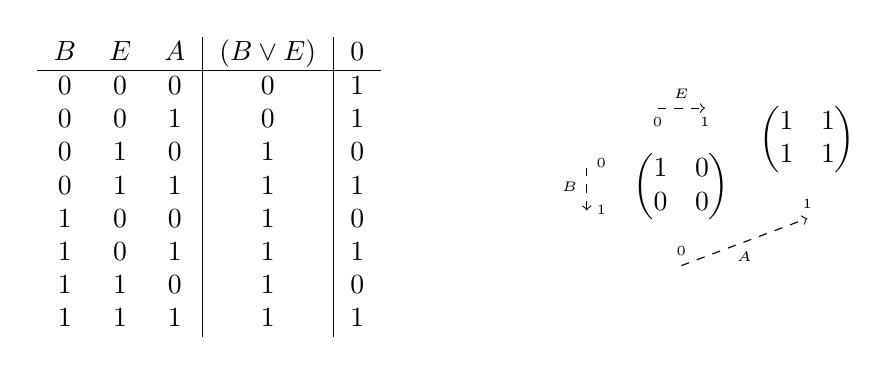
\begin{tikzpicture}[scale=2]
                    \node (tab) at (-3,0) {
                        \begin{tabular}{ccc|c|c}
                            $\catvariableof{B}$ & $\catvariableof{E}$ & $\catvariableof{A}$ & $(\catvariableof{B} \lor \catvariableof{E})$ & $\formulaof{0}$ \\
                            \hline
                            0                   & 0                   & 0                   & 0                                            & 1               \\
                            0                   & 0                   & 1                   & 0                                            & 1               \\
                            0                   & 1                   & 0                   & 1                                            & 0               \\
                            0                   & 1                   & 1                   & 1                                            & 1               \\
                            1                   & 0                   & 0                   & 1                                            & 0               \\
                            1                   & 0                   & 1                   & 1                                            & 1               \\
                            1                   & 1                   & 0                   & 1                                            & 0               \\
                            1                   & 1                   & 1                   & 1                                            & 1               \\
                        \end{tabular}
                    };

                    \node (A) at (0,0) [scale=1] {
                        $\begin{pmatrix}
                             1 & 0  \\
                             0 & 0
                        \end{pmatrix}$
                    };
                    \node (A) at (0.8,0.3) [scale=1] {
                        $\begin{pmatrix}
                             1 & 1 \\
                             1 & 1
                        \end{pmatrix}$
                    };
                    \draw[->,dashed] (-0.15,0.5) node[below] {\tiny $0$} -- (0.15,0.5) node [midway, above] {\tiny $\catvariableof{E}$} node[below] {\tiny $1$};
                    \draw[<-,dashed] (-0.6,-0.15) node[right] {\tiny $1$} -- (-0.6,0.15) node [midway, left] {\tiny $\catvariableof{B}$} node[right] {\tiny $0$};
                    \draw[->,dashed] (0,-0.5) node[above] {\tiny $0$} -- (0.8,-0.2) node [midway, below] {\tiny $\catvariableof{A}$} node[above] {\tiny $1$};
                \end{tikzpicture}
            \end{center}
            \item $\formulaof{1} = \big(\catvariableof{A} \Rightarrow (\catvariableof{M}\lor\catvariableof{J})\big)$:
            \begin{center}
                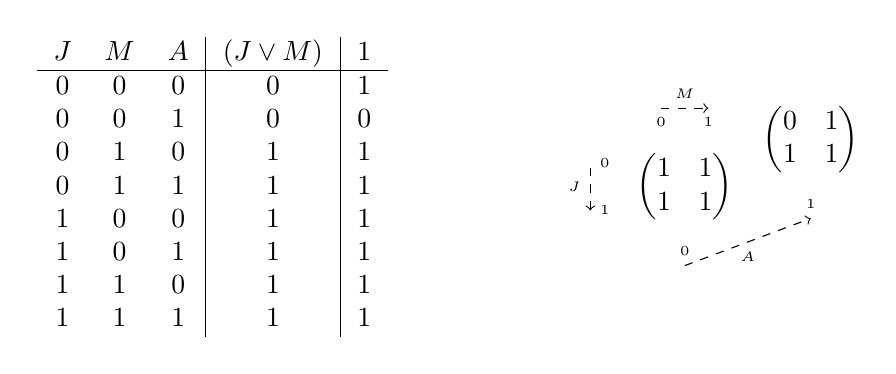
\begin{tikzpicture}[scale=2]
                    \node (tab) at (-3,0) {
                        \begin{tabular}{ccc|c|c}
                            $\catvariableof{J}$ & $\catvariableof{M}$ & $\catvariableof{A}$ & $(\catvariableof{J} \lor \catvariableof{M})$ & $\formulaof{1}$ \\
                            \hline
                            0                   & 0                   & 0                   & 0                                            & 1               \\
                            0                   & 0                   & 1                   & 0                                            & 0               \\
                            0                   & 1                   & 0                   & 1                                            & 1               \\
                            0                   & 1                   & 1                   & 1                                            & 1               \\
                            1                   & 0                   & 0                   & 1                                            & 1               \\
                            1                   & 0                   & 1                   & 1                                            & 1               \\
                            1                   & 1                   & 0                   & 1                                            & 1               \\
                            1                   & 1                   & 1                   & 1                                            & 1               \\
                        \end{tabular}
                    };

                    \node (A) at (0,0) [scale=1] {
                        $\begin{pmatrix}
                             1 & 1  \\
                             1 & 1
                        \end{pmatrix}$
                    };
                    \node (A) at (0.8,0.3) [scale=1] {
                        $\begin{pmatrix}
                             0 & 1 \\
                             1 & 1
                        \end{pmatrix}$
                    };
                    \draw[->,dashed] (-0.15,0.5) node[below] {\tiny $0$} -- (0.15,0.5) node [midway, above] {\tiny $\catvariableof{M}$} node[below] {\tiny $1$};
                    \draw[<-,dashed] (-0.6,-0.15) node[right] {\tiny $1$} -- (-0.6,0.15) node [midway, left] {\tiny $\catvariableof{J}$} node[right] {\tiny $0$};
                    \draw[->,dashed] (0,-0.5) node[above] {\tiny $0$} -- (0.8,-0.2) node [midway, below] {\tiny $\catvariableof{A}$} node[above] {\tiny $1$};
                \end{tikzpicture}
            \end{center}
            \item $\formulaof{2} = \lnot\catvariableof{J}$:
            \begin{center}
                \begin{tikzpicture}[scale=2]
                    \node (tab) at (-3,0) {
                        \begin{tabular}{c|c}
                            $\catvariableof{J}$ & $\formulaof{2}$ \\
                            \hline
                            0                   & 1               \\
                            1                   & 0
                        \end{tabular}
                    };
                    \node (A) at (0,0) [scale=1] {
                        $\begin{pmatrix}
                             1  \\
                             0
                        \end{pmatrix}$
                    };
                    \draw[<-,dashed] (-0.6,-0.15) node[right] {\tiny $1$} -- (-0.6,0.15) node [midway, left] {\tiny $\catvariableof{J}$} node[right] {\tiny $0$};
                \end{tikzpicture}
            \end{center}
        \end{itemize}
    }
    \addtask{3}{
        We define test formulas $\formula[\cdot]$ and decide entailment by investigating whether $\contraction{\kb[\cdot],\lnot\formula[\cdot]}=0$.
        \begin{itemize}
            \item "When the Alarm rings, either a Burglary or an Earthquake happened." \\
            Intuitively, this is not entailed, since the Alarm can ring without a Burglary or an Earthquake happening. \\
            Test formula:
            \begin{align*}
                \formulaofat{3}{\catvariableof{A},\catvariableof{B},\catvariableof{E}}
                =\big(\catvariableof{A}\Rightarrow(\catvariableof{B}\lor\catvariableof{E})\big)
            \end{align*}
            We construct an example state where $\kb$ is satisfied, but $\formulaof{4}$ is not satisfied:
            \begin{align*}
                (\catindexof{A},\catindexof{B},\catindexof{E},\catindexof{M},\catindexof{J}) = (1,0,0,1,0)
            \end{align*}
            We have $\kbat{\catvariableof{B}=0,\catvariableof{E}=0,\catvariableof{A}=1,\catvariableof{J}=0,\catvariableof{M}=1}=1$ since
            \begin{align*}
                &\formulaofat{0}{\catvariableof{A}=1,\catvariableof{B}=0,\catvariableof{E}=0} = 1 \\
                &\formulaofat{1}{\catvariableof{A}=1,\catvariableof{J}=0,\catvariableof{M}=1} = 1 \\
                &\formulaofat{2}{\catvariableof{J}=0} = 1
            \end{align*}
            but
            \begin{align*}
                &\formulaofat{3}{\catvariableof{A}=1,\catvariableof{B}=0,\catvariableof{E}=0} = 0 \, .
            \end{align*}
            Therefore $\contraction{\kbat{\catvariableof{B},\catvariableof{E},\catvariableof{A},\catvariableof{J},\catvariableof{M}},\lnot\formulaofat{3}{\catvariableof{A},\catvariableof{B},\catvariableof{E}}}>1$ and
            \begin{align*}
                \kb\not\models\formulaof{3} \, .
            \end{align*}
            \item "When the Alarm rings, then Mary calls." \\
            Intuitively, this already follows from the last two formulas, since when the Alarm rings, then at least one of the neighbors calls, and since John never calls, it must be Mary who calls. \\
            Test formula:
            \begin{align*}
                \formulaofat{4}{\catvariableof{A},\catvariableof{M}}
                =\big(\catvariableof{A}\Rightarrow\catvariableof{M}\big)
            \end{align*}
            We have
            \vspace{-1cm}
            \begin{center}
                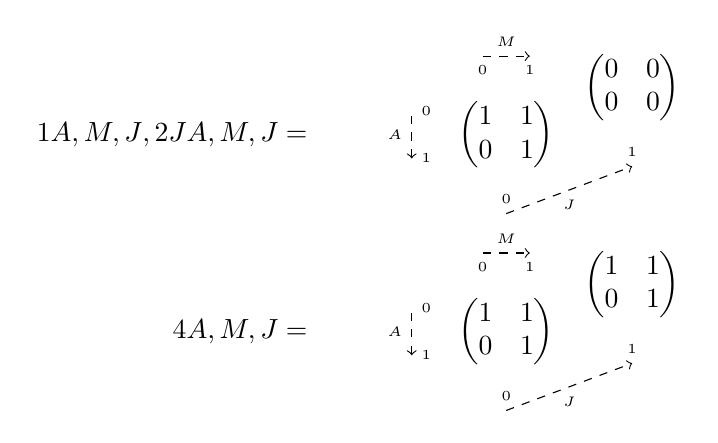
\begin{tikzpicture}[scale=2]
                    \node[anchor=east] at (-1.2,0)  {$\contractionof{\formulaofat{1}{\catvariableof{A},\catvariableof{M},\catvariableof{J}},\formulaofat{2}{\catvariableof{J}}}{\catvariableof{A},\catvariableof{M},\catvariableof{J}}=$};
                    \node (A) at (0,0) [scale=1] {
                        $\begin{pmatrix}
                             1 & 1  \\
                             0 & 1
                        \end{pmatrix}$
                    };
                    \node (A) at (0.8,0.3) [scale=1] {
                        $\begin{pmatrix}
                             0 & 0 \\
                             0 & 0
                        \end{pmatrix}$
                    };
                    \draw[->,dashed] (-0.15,0.5) node[below] {\tiny $0$} -- (0.15,0.5) node [midway, above] {\tiny $\catvariableof{M}$} node[below] {\tiny $1$};
                    \draw[<-,dashed] (-0.6,-0.15) node[right] {\tiny $1$} -- (-0.6,0.15) node [midway, left] {\tiny $\catvariableof{A}$} node[right] {\tiny $0$};
                    \draw[->,dashed] (0,-0.5) node[above] {\tiny $0$} -- (0.8,-0.2) node [midway, below] {\tiny $\catvariableof{J}$} node[above] {\tiny $1$};
                    \begin{scope}[shift={(0,-1.25)}]
                        \node[anchor=east] at (-1.2,0)  {$\formulaofat{4}{\catvariableof{A},\catvariableof{M},\catvariableof{J}}=$};
                        \node (A) at (0,0) [scale=1] {
                            $\begin{pmatrix}
                                 1 & 1  \\
                                 0 & 1
                            \end{pmatrix}$
                        };
                        \node (A) at (0.8,0.3) [scale=1] {
                            $\begin{pmatrix}
                                 1 & 1  \\
                                 0 & 1
                            \end{pmatrix}$
                        };
                        \draw[->,dashed] (-0.15,0.5) node[below] {\tiny $0$} -- (0.15,0.5) node [midway, above] {\tiny $\catvariableof{M}$} node[below] {\tiny $1$};
                        \draw[<-,dashed] (-0.6,-0.15) node[right] {\tiny $1$} -- (-0.6,0.15) node [midway, left] {\tiny $\catvariableof{A}$} node[right] {\tiny $0$};
                        \draw[->,dashed] (0,-0.5) node[above] {\tiny $0$} -- (0.8,-0.2) node [midway, below] {\tiny $\catvariableof{J}$} node[above] {\tiny $1$};
                    \end{scope}
                \end{tikzpicture}
            \end{center}
            Comparing both we have
            \begin{align*}
                \contractionof{
                    \formulaofat{1}{\catvariableof{A},\catvariableof{M},\catvariableof{J}},
                    \formulaofat{2}{\catvariableof{J}},
                    \lnot\formulaofat{4}{\catvariableof{A},\catvariableof{M},\catvariableof{J}}}{\catvariableof{A},\catvariableof{M},\catvariableof{J}}
                = \zerosat{\catvariableof{A},\catvariableof{M},\catvariableof{J}}
            \end{align*}
            where by $\zerosat{\cdot}$ we denote tensors which coordinates are always $0$.
            Including further tensors will thus also yield the tensor of $0$ coordinates, and therefore
            \begin{align*}
                \contractionof{
                    \formulaofat{0}{\catvariableof{B},\catvariableof{E},\catvariableof{A}},
                    \formulaofat{1}{\catvariableof{A},\catvariableof{M},\catvariableof{J}},
                    \formulaofat{2}{\catvariableof{J}},
                    \lnot\formulaofat{4}{\catvariableof{A},\catvariableof{M},\catvariableof{J}}}{\catvariableof{A},\catvariableof{M},\catvariableof{J}}
                = \zerosat{\catvariableof{A},\catvariableof{M},\catvariableof{J}}
            \end{align*}
            and
            \begin{align*}
                \contraction{
                    \formulaofat{0}{\catvariableof{B},\catvariableof{E},\catvariableof{A}},
                    \formulaofat{1}{\catvariableof{A},\catvariableof{M},\catvariableof{J}},
                    \formulaofat{2}{\catvariableof{J}},
                    \lnot\formulaofat{4}{\catvariableof{A},\catvariableof{M},\catvariableof{J}}}
                = 0 \, .
            \end{align*}
            We conclude that $\kb\models\formulaof{4}$.
            \item "When neither Mary nor John calls, then either the alarm did not ring, or a Burglary did not happen or an Earthquake did not happen."\\
            Test formula:
            \begin{align*}
                \formulaofat{5}{\catvariableof{B},\catvariableof{E},\catvariableof{A},\catvariableof{M},\catvariableof{J}}
                = \big((\lnot\catvariableof{M}\land\lnot\catvariableof{J})\Rightarrow(\lnot\catvariableof{A}\lor\lnot\catvariableof{B}\lor\lnot\catvariableof{E})\big)
            \end{align*}
            Trick: There is a single $0$ coordinate to $\formulaof{5}$, namely at the state
            \begin{align*}
                (\catindexof{B},\catindexof{E},\catindexof{A},\catindexof{M},\catindexof{J}) = (1,1,1,0,0) \, .
            \end{align*}
            The negation $\lnot\formulaof{5}$ has thus a single $1$ coordinate at this state.
            It follows that
            \begin{align*}
                & \contraction{
                    \kbat{\catvariableof{B},\catvariableof{E},\catvariableof{A},\catvariableof{M},\catvariableof{J}},
                    \lnot\formulaofat{5}{\catvariableof{B},\catvariableof{E},\catvariableof{A},\catvariableof{M},\catvariableof{J}}
                } \\
                &\quad= \kbat{\catvariableof{B}=1,\catvariableof{E}=1,\catvariableof{A}=1,\catvariableof{J}=0,\catvariableof{M}=0} \\
                &\quad= 0
            \end{align*}
            We used that the knowledge base $\kb$ is not satisfied at this state, since the formula $\formulaof{1}$ is violated.
            We conclude that $\kb\models\formulaof{5}$.
        \end{itemize}
    }
\end{document}